\begin{figure*}[t!]
\begin{centering}
	\begin{subfigure}[b]{0.23\textwidth}
                \centering
                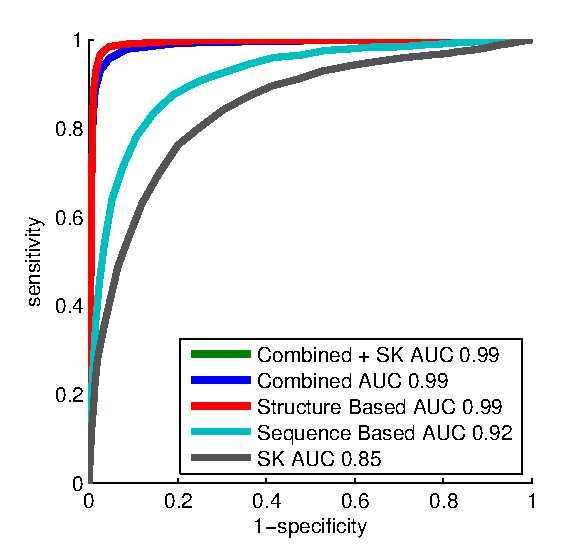
\includegraphics[width=\textwidth]{Figures/vq/SCOP_ROC/all_alpha_ROC}
                \caption{Alll $\alpha$}
                \label{fig:ocS1A}
        \end{subfigure}%
        \quad
	\begin{subfigure}[b]{0.23\textwidth}
                \centering
                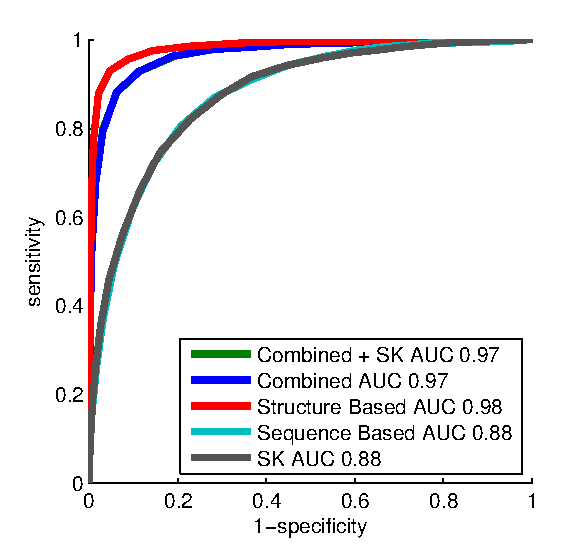
\includegraphics[width=\textwidth]{Figures/vq/SCOP_ROC/all_beta_ROC}
                \caption{All $\beta$}
                \label{fig:ocS1B}
        \end{subfigure}
	\quad
	\begin{subfigure}[b]{0.23\textwidth}
                \centering
                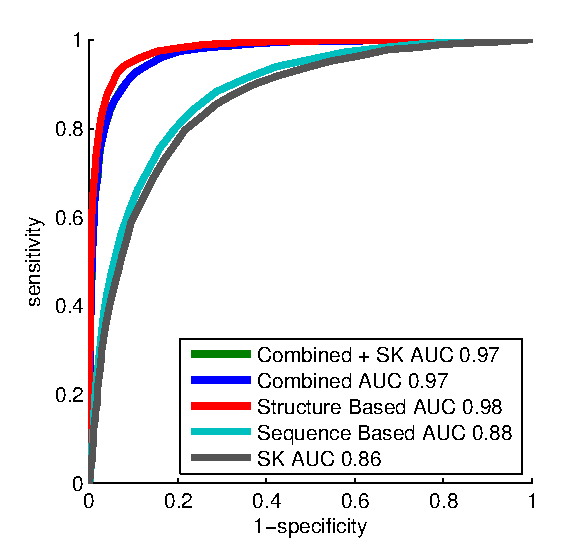
\includegraphics[width=\textwidth]{Figures/vq/SCOP_ROC/alpha_div_beta_ROC}
                \caption{$\alpha$/\ $\beta$}
                \label{fig:ocS1A}
        \end{subfigure}%
        \quad
	\begin{subfigure}[b]{0.23\textwidth}
                \centering
                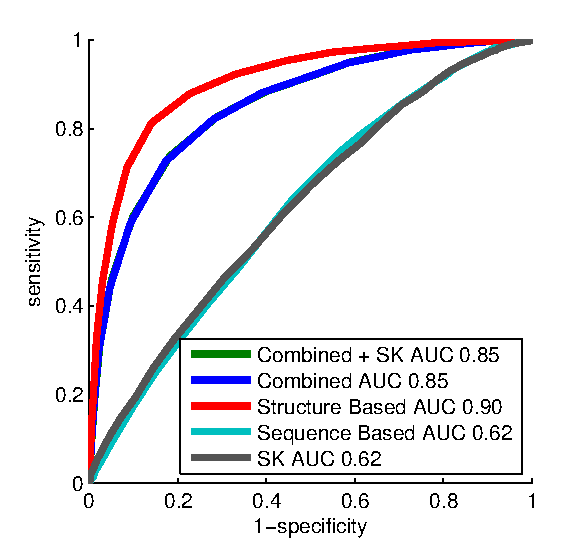
\includegraphics[width=\textwidth]{Figures/vq/SCOP_ROC/alpha_plus_beta_ROC}
                \caption{$\alpha$ + $\beta$}
                \label{fig:ocS1B}
        \end{subfigure}

\end{centering}
\caption[SCOP ROC curves]{SCOP ROC curves showing the performance of each combination of combined features and the string kernel when predicting each category of SCOP fold tested.}
\label{fig:SCOP_ROC}
\end{figure*}




%%%%%%%%%%%%%%%%%%%%%%
%%%%%%%%%%%%%%%%%%%%%%

%\begin{figure*}[t!]
%\begin{centering}
%	\begin{subfigure}[b]{0.35\textwidth}
%                \centering
%                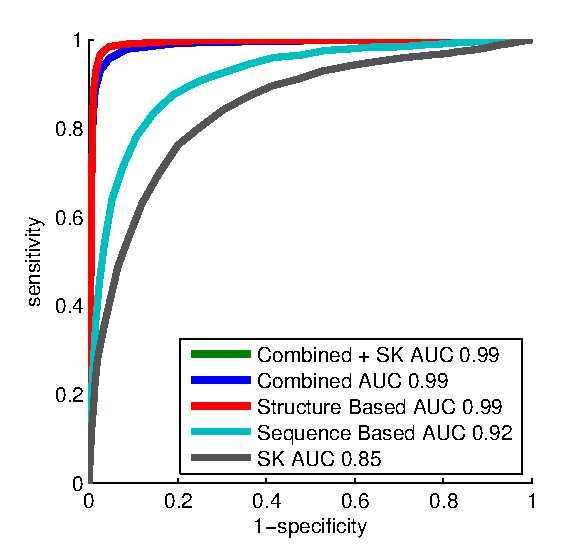
\includegraphics[width=\textwidth]{Figures/vq/SCOP_ROC/all_alpha_ROC}
%                \caption{Alll $\alpha$}
%                \label{fig:ocS1A}
%        \end{subfigure}%
%        \quad
%        \quad
%        \quad
%	\begin{subfigure}[b]{0.35\textwidth}
%                \centering
%                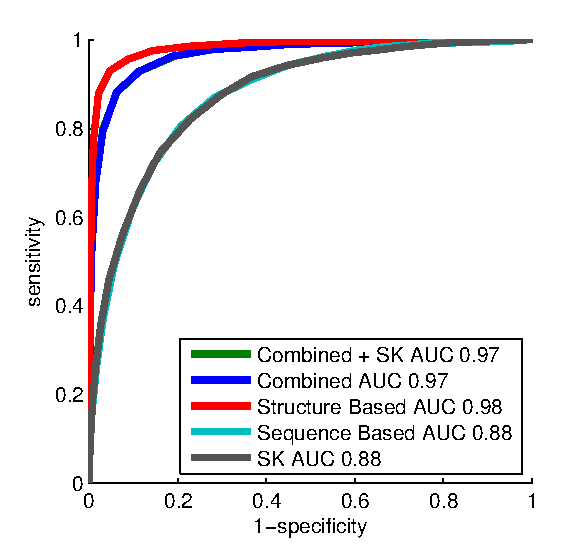
\includegraphics[width=\textwidth]{Figures/vq/SCOP_ROC/all_beta_ROC}
%                \caption{All $\beta$}
%                \label{fig:ocS1B}
%        \end{subfigure}
%
%	\begin{subfigure}[b]{0.35\textwidth}
%                \centering
%                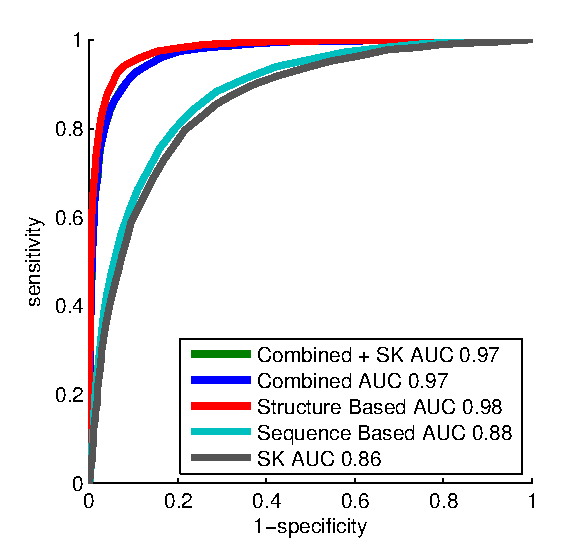
\includegraphics[width=\textwidth]{Figures/vq/SCOP_ROC/alpha_div_beta_ROC}
%                \caption{$\alpha$/\ $\beta$}
%                \label{fig:ocS1A}
%        \end{subfigure}%
%        \quad
%        \quad
%        \quad
%	\begin{subfigure}[b]{0.35\textwidth}
%                \centering
%                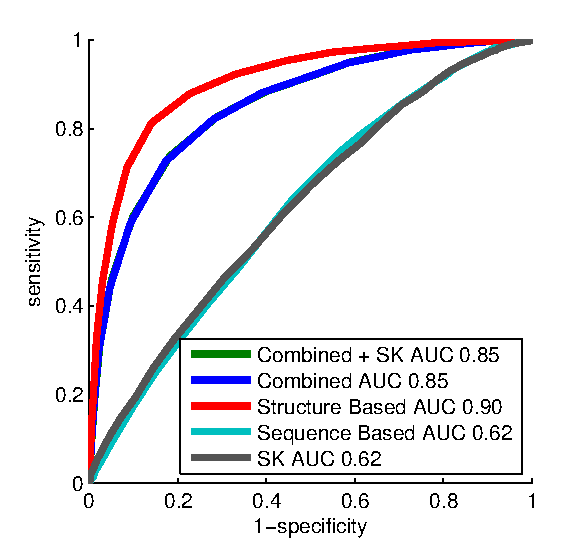
\includegraphics[width=\textwidth]{Figures/vq/SCOP_ROC/alpha_plus_beta_ROC}
%                \caption{$\alpha$ + $\beta$}
%                \label{fig:ocS1B}
%        \end{subfigure}
%
%\end{centering}
%\caption[SCOP ROC Curves]{SCOP ROC Curves showing the performance of each combination of combined features and the string kernel when predicting each category of SCOP fold tested.}
%\label{fig:SCOP_ROC}
%\end{figure*}

%%%%%%%%%%%%%%%%%%%%%%
%%%%%%%%%%%%%%%%%%%%%%